\chapter{Introduction to normal mixture models}% Umlaute work thanks to \inputencoding{..} % in main file

here intro to normal mixtures

A good and thorough introductory book is the work of McLachlan and Peel 2000 and
the reader is encouraged to study that to learn in depth about normal mixtures. 
We will here give a short overwiev of normal mixtures to fix notation and nomenclature.

Let $ \mu \in \mathbb{R}^p , \quad \Sigma \in \mathbb{R}^{p \times p} $ and 
$ \phi(\mu, \Sigma) $ be the normal distribution with
mean $ \mu $ and covariance matrix $ \Sigma $.

Normal mixture model are designed for situations where we assume that a given 
dataset originates from more than one population of explaining variables.

$ \pmb{Y}_1, \dots , \pmb{Y}_n $

\begin{definition}
	Suppose we have a random sample $ \pmb{Y}_1, \dots , \pmb{Y}_n $ with 
	probability density function $ \pmb{Y}_j \sim f(y_j) $ on $\mathbb{R}^p$
	We assume that the density $ f(y_j) $ of $ \pmb{Y}_j $ can be written in
	the form 

	\[ f(y_j) = \sum_{i=1}^{K} \pi_i \phi_i (y_i) \]

	The $ \pi_i $ are called the component densities of the mixture.
\end{definition}

explain in scetch EM algo

explain idea to use parameter optimizer instead,
EM has pathological insufficiencies, like 'getting stuck' for many iterations.
we hope we need less iterations, and as concequence less time.
'special' idea: using cholesky decomp.


\section{choice of notation}

describe difference in notation between ceuleux \& govaert and our covariance matrix decomposition.

The classification of models in this paper relies heavily on the work of Celeux and Grovaert,
however, out of necessity for clarity, we break with their notation. 
So as to not confuse the reader we describe here in depth the differences in notation
between Celeux and Govaert and ours.

explanation for the volume, shape and orientation descriptors

The basis of classification in CnG is the decomposition of a symmetric matrix into
an orthogonal and a diagonal component.
A symmetric positive definite matrix $ \Sigma $ can be decomposed as follows
\[ \Sigma = \lambda \pmb{D} \pmb{A} \pmb{D}^{\top} \]
with $ \pmb{D} $ an orthogonal matrix and $ \pmb{A} $ a diagonal matrix and 
$ \lambda = \sqrt[\uproot{3}p]{det(\Sigma)} $ the $ p-th $ root of the determinant 
of $ \Sigma $.

This decomposition has an appealing geometric interpretation, with $ \pmb{D} $ 
as the \textit{orientation} of the distribution, $ \pmb{A} $ the \textit{shape}, and $ \lambda $
the \textit{volume}.
The problem of notation comes from standard conventions in linear algebra, where
the letters $A$ and $D$ are usually occupied by arbytrary and diagonal matrices 
respectively. Furthermore, we intend to apply a variant of the Cholesky decomposition
to $ \Sigma $, the $ \pmb{L}\pmb{D}\pmb{L}^{\top} $ decomposition.
This obviously raises some conflicts in notation.

Therefore we, from here on, when reffering to the decomposition as described
by cng, will use the following modification of notation:

\begin{align*} 
	\pmb{D} \longmapsto \pmb{Q} \\
	\pmb{A} \longmapsto \pmb{\Lambda} \\
	\lambda \longmapsto \alpha  \\
	\Sigma = \lambda \pmb{D} \pmb{A} \pmb{D}^{\top} =
		\alpha \pmb{Q} \pmb{\Lambda} \pmb{Q}^{\top}
\end{align*}

These were chosen according to general conventions of linear algebra.
$ \pmb{Q} $ is usually chosen for orthonormal matrices; $ \pmb{\Lambda} $ is 
often a choice for eigen vectors and $ \alpha $ was somewhat arbitrarily chosen.


make clear that the models can not be translated one to one to ldlt model

make nice table(maybe sideways to account for parameter list)


\begin{table}[!htb]
	\centering
\rotatebox{90}
{
	\begin{tabular}{| c | c c c c c c | c c c |}
		\hline
		Model & $\pmb{\Sigma}_k$ C\&G & volume & shape & orientation & parameters & count & $ \pmb{LDL}^\top $ & parameters & count \\
		\hline

		EII	& $ \alpha \pmb{I} $ & equal & equal & - & $ \alpha $ 
				& 1 & same as C\&G
						& & \\

		VII	& $ \alpha_k \pmb{I} $ 		& variable & equal & - & $ \alpha_k $ 
				& $ K $ &
					& & \\

		EEI	& $ \alpha \pmb{\Lambda} $ 	& equal & equal & coordinate axes & $ \alpha, \lambda_i $ 
				& $ 1+p $ &
					& & \\

		VEI	& $ \alpha_k \pmb{\Lambda} $ & variable & equal & coordinate axes & $ \alpha_k, \lambda_{i}$ 
				& $ K+p $ &
					& & \\

		EVI	& $ \alpha \pmb{\Lambda}_k $ &equal & variable & coordinate axes & $ \alpha, \lambda_{i,k} $ 
				& $ 1+pK $ &
					& & \\

		VVI	& $ \alpha_k \pmb{\Lambda}_k $ & variable & variable & coordinate axes & $ \alpha_k, \lambda_{i,k} $ 
				& $ K+pK $ &
					& & \\

		\hline

		EEE	& $ \alpha \pmb{Q \Lambda Q}^\top $ &equal & equal & equal & $ \alpha, \lambda_{i}, q_{i,j} $ 
				& $ 1+p+p^2 $ & don't exist
					& & \\

		EVE	& $ \alpha \pmb{Q \Lambda}_k \pmb{Q}^\top $ &equal & variable & equal & $ \alpha, \lambda_{i,k}, q_{i,j} $ 
				& $ 1+pK+p^2 $ &
					& & \\

		VEE	& $ \alpha_k \pmb{Q \Lambda Q}^\top $ & variable & equal & equal & $ \alpha_k, \lambda_{i}, q_{i,j} $ 
				& $ K+p+p^2 $ &
					& & \\
					
		VVE	& $ \alpha_k \pmb{Q \Lambda}_k \pmb{Q}^\top $ &variable & variable & equal & $ \alpha_k, \lambda_{i,k}, q_{i,j} $ 
				& $ K+pK+p^2 $ &
					& & \\

		EEV	& $ \alpha \pmb{Q}_k \pmb{\Lambda} \pmb{Q}_k^\top $ &equal & equal & variable & $ \alpha, \lambda_{i}, q_{i,j,k} $ 
				& $ 1+p+Kp^2 $ &
					& & \\

		VEV	& $ \alpha_k \pmb{Q}_k \pmb{\Lambda} \pmb{Q}_k^\top $ &variable & equal & variable & $ \alpha_k, \lambda_{i}, q_{i,j,k} $ 
				& $ K+p+Kp^2 $ &
					& & \\

		\hline

		EVV	& $ \alpha \pmb{Q}_k \pmb{\Lambda}_k \pmb{Q}_k^\top $ & equal & variable & variable & $ \alpha, \lambda_{i}, q_{i,j,k} $ 
				& $ 1+pK+Kp^2 $ & $ \alpha \pmb{L}_k \pmb{D}_k \pmb{L}_k^\top $ 
					& $ \lambda, d_{i,k}, l_{i,j,k}\ j>i $ & $ 1+pK+K\frac{p(p-1)}{2} $ \\

		VVV	& $ \alpha_k \pmb{Q}_k \pmb{\Lambda}_k \pmb{Q}_k^\top $ & variable & variable & variable & $ \alpha_k, \lambda_{i}, q_{i,j,k} $ 
				& $ K+pK+Kp^2 $ & $ \alpha_k \pmb{L}_k \pmb{D}_k \pmb{L}_k^\top $ 
					& $ \lambda_k, d_{i,k}, l_{i,j,k}\ j>i $ & $ K+pK+K\frac{p(p-1)}{2} $ \\

		\hline

	\end{tabular}

	\label{table:1}

}

\caption{Table of Parameters}

\end{table}


\clearpage

\section{problems of EM}


the EM algo has stalling problems especially close to a local optimum

show an example using nor1mix


\begin{Schunk}
\begin{Sinput}
> library("nor1mix")
> plot(MW.nm9, lty=2, col = "blue", p.norm=FALSE, p.comp=TRUE)
> set.seed(2019)
> x9 <- rnorMix(5000, MW.nm9)
> lines(density(x9), lwd=1.8)# "clearly" 3 components
\end{Sinput}
\end{Schunk}
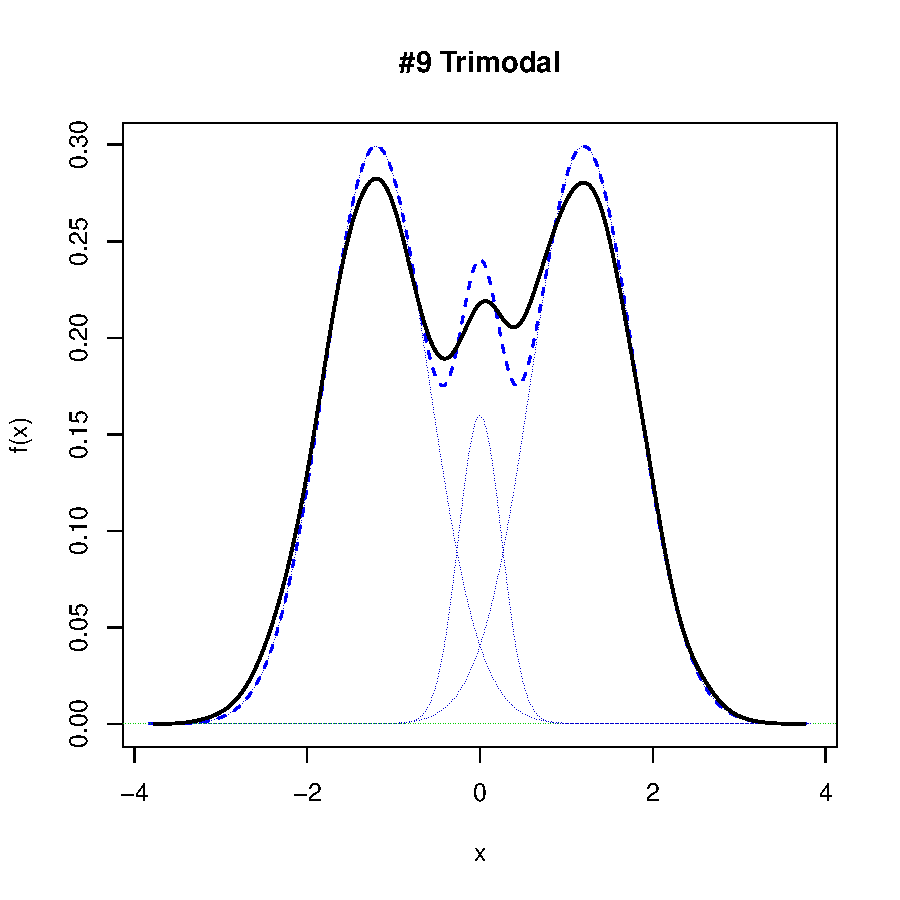
\includegraphics{chapter1-001}


then an illustration of MW examples of pathological cases


\begin{Schunk}
\begin{Sinput}
> p.EMsteps <- function(nSteps, x, nmObj,
+                       main = "EM for 1-dim normal mixtures",
+                       sleep = nSteps <= 40, sec.sleep = 0.2, col2 = "tomato",
+                       showLik = nSteps <= 80,
+                       plotIni = FALSE, # plot the initial param. ?
+                       doNote = TRUE)
+ {
+     ## Purpose: show progress of EM - steps -- only few steps
+     ## ----------------------------------------------------------------------
+     ## Author: Martin Maechler, Date: 26 Nov 2009
+     stopifnot(is.norMix(nmObj), is.numeric(x), nSteps >= 1)
+     nm. <- nmObj
+     ll.em <- numeric(nSteps)
+     for(k in 1:nSteps) {
+         z. <- estep.nm(x9, obj = nm.)
+         nm. <- do.call(norMix, c(mstep.nm(x=x9, z=z.), name=""))
+         if(k == 1) { ## only after the first E+M - step
+             op <- par(mar = c(0,0,0, 2.) + par("mar")); on.exit(par(op))
+             plot(nm., p.norm=FALSE, main = main)
+             if(plotIni) lines(nmObj, p.norm=FALSE)
+             rug(x) ; mtext(paste("n = ", length(x)),
+                            line = -1., adj=.99)
+             nm2 <<- nm. ## save the 2nd
+             if(showLik) {
+                 yVal <- approxfun(x=c(nSteps,1), y=par("usr")[3:4])
+                 xV <- { u <- par("usr")[1:2]; u[2] + .01*(u[2]-u[1]) }
+             }
+         } else lines(nm., p.norm=FALSE, col = rgb(0,0,0, 0.2))
+         print(ll <- llnorMix(nM2par(nm.), x=x9))
+         ll.em[k] <- ll
+         if(showLik)
+             text(xV, yVal(k), sprintf("%3d: %5.1f", k, ll),
+                  cex = 0.8, adj = 0, xpd = NA)
+         if(sleep) Sys.sleep(sec.sleep)
+     }
+     ## plot the last one more visibly
+     lines(nm., p.norm=FALSE, col = col2, lwd = 2)
+     if(doNote)
+         mtext(paste(nSteps," E-, M-steps seem to have converged nicely .."),
+               col=col2)
+     ## return final normal mixture {but invisibly}:
+     invisible(list(nm = nm., logLik = ll.em))
+ }
> 
\end{Sinput}
\end{Schunk}

here figure maybe

\begin{figure}
\begin{Schunk}
\begin{Sinput}
> clp0 <- cluster::clara(x9, k=3, samples=1000, medoids.x = FALSE, rngR=TRUE)
> nm1 <- clus2norMix(clp0$clustering, x9) ## <-- M-step from cluster:
> p.EMsteps(20, x9, nm1, plotIni=TRUE)# 20 steps: final logLik ("ll"): -7779.5
\end{Sinput}
\begin{Soutput}
[1] -7881.319
[1] -7864.054
[1] -7857.641
[1] -7854.718
[1] -7853.212
[1] -7852.369
[1] -7851.864
[1] -7851.543
[1] -7851.327
[1] -7851.173
[1] -7851.055
[1] -7850.961
[1] -7850.88
[1] -7850.808
[1] -7850.742
[1] -7850.679
[1] -7850.617
[1] -7850.557
[1] -7850.498
[1] -7850.439
\end{Soutput}
\begin{Sinput}
> 
\end{Sinput}
\end{Schunk}
\end{figure}


